\documentclass[conf]{new-aiaa}
%\documentclass[journal]{new-aiaa} for journal papers

% Package Imports
\usepackage{csvsimple}
\usepackage{graphicx}
\usepackage{amsmath, amssymb}
\usepackage{siunitx}
\usepackage{listings}
\usepackage{xcolor}
\usepackage{booktabs}
\usepackage{float}
\usepackage[utf8]{inputenc}
\usepackage{listings}
\usepackage{float}
\usepackage{graphicx}
\usepackage{amsmath}
\usepackage[version=4]{mhchem}
\usepackage{siunitx}
\usepackage{longtable,tabularx}
\setlength\LTleft{0pt} 

% Title & Author
\title{Lab 6 - Round Jet PIV Measurement}
\author{Parham Khodadi\footnote{Aerospace Engineering student, San Diego State University}}
\affil{A E 303, Section 3, with Dr. Xiaofeng Liu}

\lstdefinestyle{pythonstyle}{
    language=Python,
    basicstyle=\ttfamily\footnotesize,
    keywordstyle=\color{blue},
    commentstyle=\color{gray},
    stringstyle=\color{orange},
    breaklines=true,
    breakatwhitespace=true,
    tabsize=4,
    frame=single,
    numbers=left,
    numberstyle=\tiny\color{gray}
}

\begin{document}

\maketitle

\begin{abstract}
This experiment aimed to investigate the flow characteristics of a turbulent round jet using Particle Image Velocimetry (PIV). The EduPIV system was used to capture high-resolution velocity fields by tracking tracer particles in a water tank, illuminated by an LED light sheet and recorded by a camera connected to DynamicStudio. The collected data were processed in MATLAB to compute time-averaged velocities, Reynolds stresses, and vorticity. Results revealed a well-defined shear layer and the onset of turbulence downstream of the nozzle. Challenges included particle seeding uniformity and lighting consistency. Overall, the experiment successfully demonstrated key PIV principles and provided insight into turbulent jet behavior.
\end{abstract}


\section{Nomenclature}
{\renewcommand\arraystretch{1.0}
\noindent\begin{longtable*}{@{}l @{\quad=\quad} l@{}}
\(\bar{u}, \bar{v}\) & Time-averaged streamwise and cross-stream velocities (m/s) \\
\(u', v'\) & Velocity fluctuations in \(x\) and \(y\) directions (m/s) \\
\(u'^2, v'^2\) & Reynolds normal stresses (m\(^2\)/s\(^2\)) \\
\(u'v'\) & Reynolds shear stress (m\(^2\)/s\(^2\)) \\
\(\omega_z\) & Spanwise vorticity (1/s) \\
\(X, Y\) & Spatial coordinates in the measurement plane (mm) \\
\(D\) & Nozzle diameter (mm) \\
\(x/D, y/D\) & Non-dimensional streamwise and cross-stream coordinates (–) \\
\end{longtable*}}

\section{Introduction}
This lab aimed to investigate the turbulent structure of a round jet using Particle Image Velocimetry (PIV). PIV enables non-intrusive measurement of fluid velocity fields by tracking the motion of seeded particles illuminated by a light sheet. The experiment focused on visualizing and quantifying jet development, shear layer growth, and turbulence characteristics. Using the EduPIV system, flow images were captured, analyzed in DynamicStudio, and further processed in MATLAB to obtain time-averaged velocities, Reynolds stresses, and vorticity.

\section{Theory}
\label{sec:theory}

The goal of this experiment was to study the near-field behavior of a free, round turbulent jet using Particle Image Velocimetry (PIV), a modern optical measurement technique that has transformed experimental fluid dynamics \cite{liu2025piv}. Compared to older pointwise methods like Pitot tubes or Laser Doppler Velocimetry (LDV), PIV enables non-intrusive, planar velocity measurements by tracking seeding particles illuminated by a laser sheet across consecutive images \cite{zhao2010piv,anderson2017fundamentals}. With a sufficiently high acquisition rate and particle density, PIV captures detailed instantaneous velocity fields in space and time.

In this lab, the EduPIV system was used to investigate the velocity structure and turbulence characteristics of a round jet in water. Velocity vectors were extracted using Dantec DynamicStudio and exported as a series of 300 CSV files—each capturing a time step. These files were post-processed in MATLAB to produce time-averaged velocity fields, Reynolds stresses, and vorticity maps \cite{matlab}.

To analyze turbulence, Reynolds decomposition was applied to the velocity fields. The instantaneous streamwise and cross-stream velocities $u(t)$ and $v(t)$ were decomposed into time-averaged components and fluctuations as follows:

\begin{align}
u(t) &= \bar{u} + u'(t) \\
v(t) &= \bar{v} + v'(t)
\end{align}

The fluctuations $u'$ and $v'$ represent the unsteady portion of the flow. From these, Reynolds stresses were computed to quantify the turbulence intensity and shear:

\begin{align}
\overline{u'^2} &: \text{Reynolds normal stress in the } x \text{ direction} \\
\overline{v'^2} &: \text{Reynolds normal stress in the } y \text{ direction} \\
\overline{u'v'} &: \text{Reynolds shear stress}
\end{align}

These stresses represent the turbulent transport of momentum and appear as additional terms in the Reynolds-Averaged Navier-Stokes (RANS) equations \cite{liu2003reynolds}. 

To characterize rotational structures and vortex formation, 2D spanwise vorticity $\omega_z$ was calculated using the velocity gradients:

\begin{equation}
\omega_z = \frac{\partial v}{\partial x} - \frac{\partial u}{\partial y}
\end{equation}

This helped identify regions of shear and rotational motion, particularly in the shear layer surrounding the jet core.

According to previous studies \cite{mattingly1962round, cooper2004round}, round jets exhibit a potential core near the nozzle and develop shear-layer instabilities that grow into turbulence. These instabilities can be axisymmetric or helical, and their evolution is governed by the Reynolds number and boundary conditions.

In this lab, MATLAB was used to automate the processing of raw data, including averaging, interpolating onto a uniform grid, and calculating stresses and vorticity using gradient-based methods. The uniform grid enabled consistent contour and profile plotting, making it easier to identify jet structure and compare locations nondimensionalized by nozzle diameter $D$.

\subsection*{Sample Calculation Reference}
A step-by-step calculation for time-averaged velocity is included in Appendix B. This uses one vector point from a raw CSV file and applies the same logic used in the MATLAB processing script to compute $\bar{u}$ and $\bar{v}$. The values used are directly from \texttt{EduPIV\_lab.62tbxosb.000000.csv}, and the method aligns with the code shown in \texttt{ImportData\_EduPIV.m} \cite{matlab}.


\section{Experimental Setup}
\label{sec:setup}

The experiment was conducted using the EduPIV system by Dantec Dynamics to analyze a free turbulent round jet in a controlled environment. A schematic of the setup is shown in Figure~\ref{fig:schematic}, while real images of the physical layout are provided in Figures~\ref{fig:zoomedin} and~\ref{fig:zoomedout}.

\begin{figure}[H]
    \centering
    \includegraphics[width=0.95\linewidth]{Graphic.jpeg}
    \caption{Schematic of the EduPIV round jet experiment setup.}
    \label{fig:schematic}
\end{figure}

The system consists of a transparent water tank, a 3D printed round nozzle (exit diameter 5 cm), and a controlled pump for steady flow generation. Seeding particles were added to the water to enable velocity field measurements via PIV. Illumination was provided by a Dantec LED light source, which projected a 4 mm thick light sheet through fiber optics and optics modules. This light sheet illuminated the seeding particles within the measurement plane.

A Dantec FlowSense USB camera (2M-165) captured sequential images of the particle movement. The camera featured a 35 mm low-distortion lens and was positioned perpendicularly to the flow direction. All image acquisition and PIV analysis were performed using \textit{DynamicStudio} software.

\begin{figure}[H]
    \centering
    \includegraphics[width=0.7\linewidth, angle=-90]{setup_zoomedin.JPG}
    \caption{Close-up of the nozzle and flow field during operation.}
    \label{fig:zoomedin}
\end{figure}

\begin{figure}[H]
    \centering
    \includegraphics[width=0.95\linewidth]{setup_zoomedout.JPG}
    \caption{Full experimental setup showing the water tank, camera, optics, and pump system.}
    \label{fig:zoomedout}
\end{figure}

\subsection*{Materials and Equipment}

The components used in the experiment are summarized in Table~\ref{tab:equipment}. All parts are manufactured or supplied by Dantec Dynamics unless otherwise noted.

\begin{table}[H]
    \centering
    \caption{Equipment and Materials Used}
    \label{tab:equipment}
    \begin{tabular}{p{5cm} p{9cm}}
        \toprule
        \textbf{Component} & \textbf{Description} \\
        \midrule
        DynamicStudio Software & Used for image acquisition and PIV vector field computation \\
        FlowSense USB 2M-165 Camera & 1920x1200 resolution, 160 fps, USB 3.0 \\
        35mm Low-Distortion Lens & Adjustable aperture, C-mount \\
        EduPIV LED Light Source & 150W LED with fiber optic light sheet generation \\
        Optics Module & 7.6 cm wide, 35° divergence angle, 4 mm sheet thickness \\
        Seeding Particles & Polyamide particles, 50 µm diameter, 1.03 g/cm³ \\
        3D Printed Round Nozzle & 5 cm diameter, submerged in tank \\
        Flow Loop Tank & 80 × 35 × 40 cm, 112 L capacity \\
        EcoDrift 8.1 Pump & 1600–8000 L/hr, 8–20 W, speed-controlled \\
        Black Backdrop & Used to improve contrast and reduce reflection \\
        \bottomrule
    \end{tabular}
\end{table}


\section{Experimental Procedure}
\label{sec:procedure}

This experiment followed a structured procedure to ensure repeatability and data quality across all phases: preparation, calibration, and execution. The procedure was carried out using the EduPIV system in conjunction with DynamicStudio software.

\subsection*{Preparation Phase}
\begin{enumerate}
    \item The tank was filled with tap water and the nozzle was mounted horizontally inside the tank using a magnetic pump attachment.
    \item The fiber optic cable was connected to the LED light source to form a planar light sheet.
    \item Seeding particles were suspended in a test tube with water and rubbing alcohol to break the surface tension and were mixed into the tank.
    \item The camera was mounted approximately 19 cm from the tank and connected to the computer via USB.
    \item DynamicStudio was launched. The light source was set to full power and room lights were turned off.
    \item The optics were adjusted to produce a ~4 mm thick light sheet, and a black backdrop was placed at the tank’s rear wall to minimize reflections.
    \item The camera was oriented perpendicular to the flow and aligned parallel to window orientation to minimize glare.
\end{enumerate}

\subsection*{Calibration Phase}
\begin{enumerate}
    \item A calibration target was placed in the plane of the light sheet and viewed through the camera.
    \item Camera settings were adjusted (750 µs exposure, reduced frame rate) to clearly capture the target.
    \item 20 calibration images were acquired and saved in DynamicStudio.
    \item These calibration images were averaged to determine the pixel-to-mm scale factor.
\end{enumerate}

\subsection*{Execution Phase}
\begin{enumerate}
    \item The room lights were turned off again and the pump was set to a low speed for 5–10 minutes to allow flow stabilization.
    \item The camera was reset to a 150 Hz trigger rate and 750 µs exposure time.
    \item At least 300 images were recorded to ensure temporal averaging, leveraging the assumption of ergodicity for turbulent flow.
    \item The captured image pairs were processed using Adaptive PIV analysis in DynamicStudio with:
    \begin{itemize}
        \item Minimum window size: 32×32 pixels
        \item Maximum window size: 64×64 pixels
        \item 50\% overlap (16-pixel step)
    \end{itemize}
    \item The resulting velocity vector fields were exported as .csv files and imported into MATLAB for time-averaging, Reynolds stress computation, vorticity analysis, and visualization.
\end{enumerate}


\section{Results and Data Reduction}
\label{sec:results}

This section presents time-averaged and statistical flow quantities derived from planar PIV measurements of a round turbulent jet. Results include velocity contours, mean velocity profiles, Reynolds stress distributions, and vorticity characteristics.

\begin{figure}[H]
    \centering
    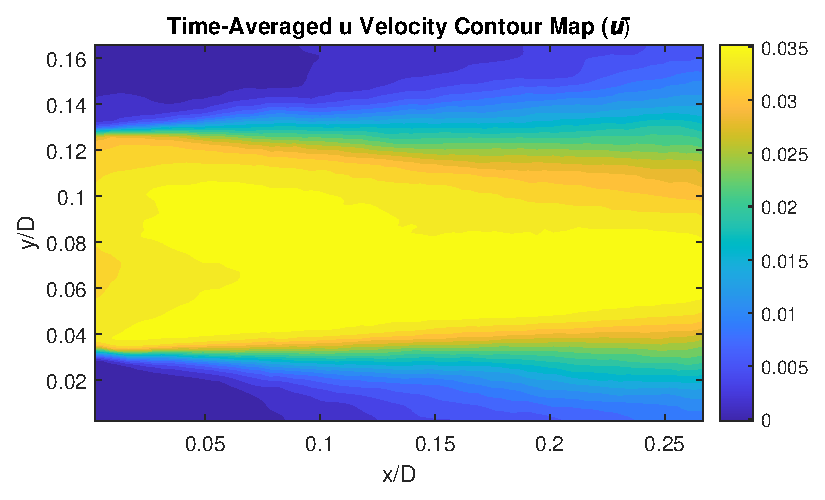
\includegraphics[width=0.95\textwidth]{u_mean_contour.eps}
    \caption{Time-averaged streamwise velocity contour map, $\bar{u}$, showing the development of the jet.}
    \label{fig:u_mean_contour}
\end{figure}

\begin{figure}[H]
    \centering
    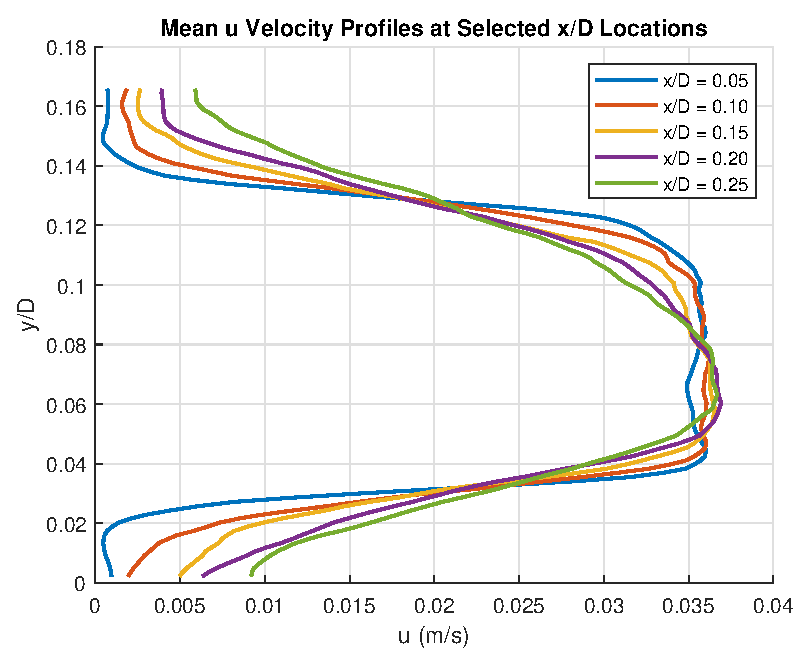
\includegraphics[width=0.9\textwidth]{u_profiles_vs_y.eps}
    \caption{Streamwise velocity profiles ($\bar{u}$) at different $x/D$ locations.}
    \label{fig:u_profiles}
\end{figure}

\begin{figure}[H]
    \centering
    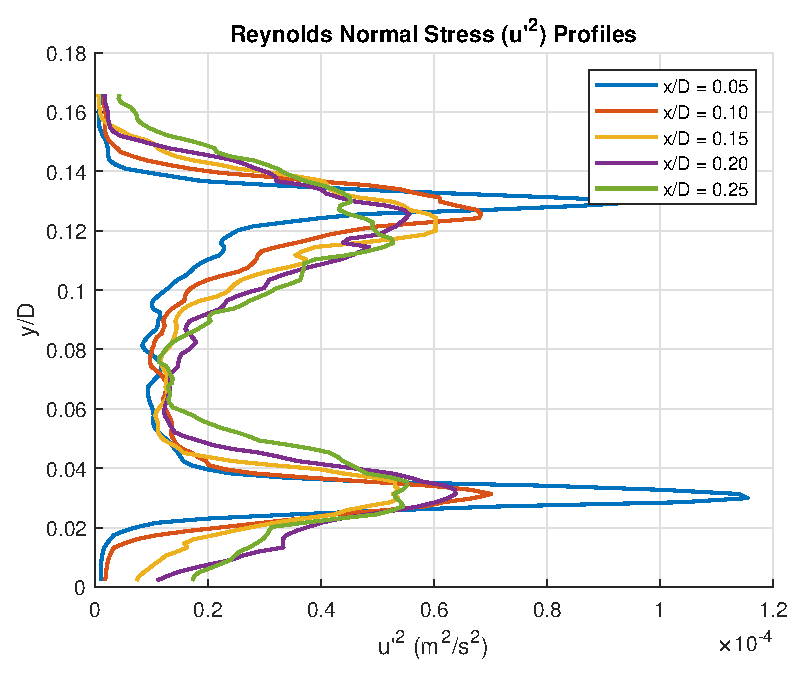
\includegraphics[width=0.9\textwidth]{uu_profiles_vs_y.eps}
    \caption{Reynolds normal stress profiles in the $x$ direction, $\overline{u'^2}$, at multiple $x/D$ stations.}
    \label{fig:uu_profiles}
\end{figure}

\begin{figure}[H]
    \centering
    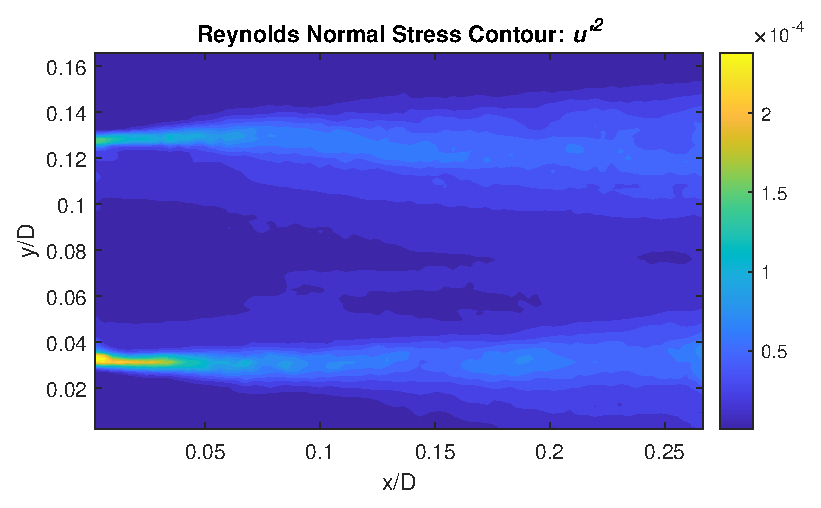
\includegraphics[width=0.95\textwidth]{uu_reynolds_normal_stress.eps}
    \caption{Contour map of $\overline{u'^2}$ revealing the extent and peak intensity of streamwise turbulence.}
    \label{fig:uu_contour}
\end{figure}

\begin{figure}[H]
    \centering
    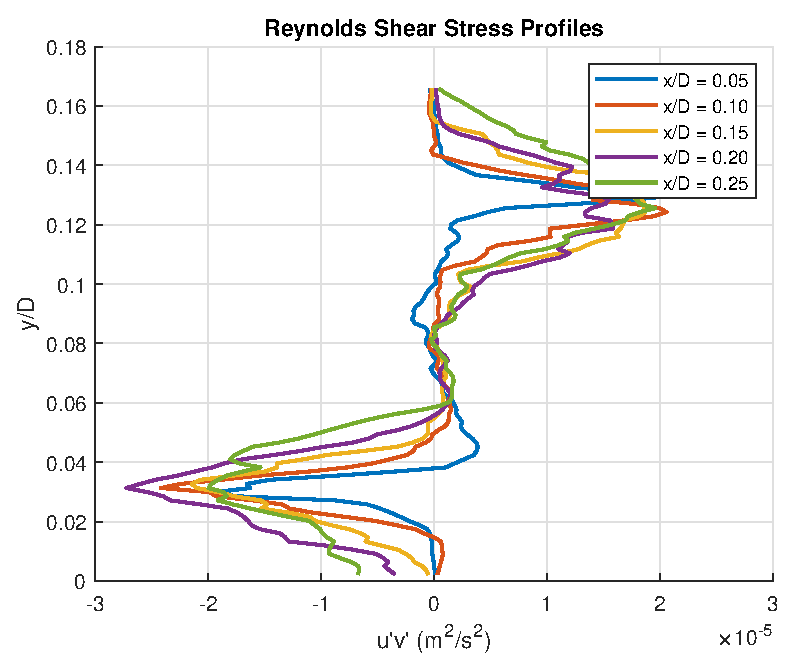
\includegraphics[width=0.9\textwidth]{uv_profiles_vs_y.eps}
    \caption{Reynolds shear stress profiles ($\overline{u'v'}$) at selected streamwise locations.}
    \label{fig:uv_profiles}
\end{figure}

\begin{figure}[H]
    \centering
    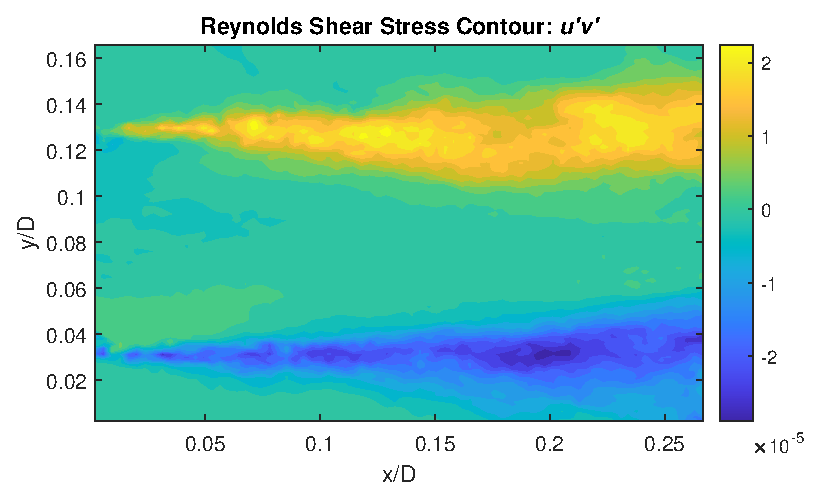
\includegraphics[width=0.95\textwidth]{uv_reynolds_shear_stress.eps}
    \caption{Reynolds shear stress contour map, $\overline{u'v'}$, indicating shear layer development.}
    \label{fig:uv_contour}
\end{figure}

\begin{figure}[H]
    \centering
    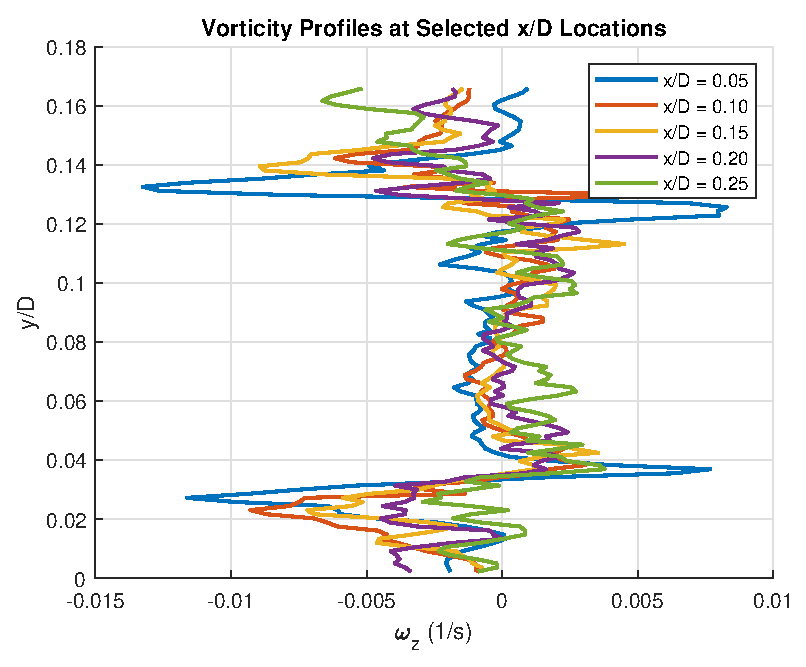
\includegraphics[width=0.9\textwidth]{vorticity_profiles_vs_y.eps}
    \caption{Vorticity profiles ($\omega_z$) at various $x/D$ locations.}
    \label{fig:vorticity_profiles}
\end{figure}

\begin{figure}[H]
    \centering
    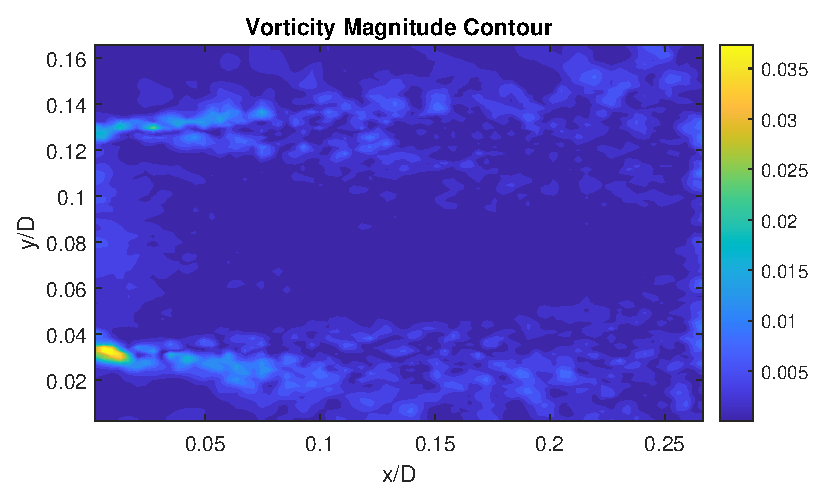
\includegraphics[width=0.95\textwidth]{vorticity_magnitude.eps}
    \caption{Contour plot of vorticity magnitude, $\left|\omega_z\right|$, highlighting regions of rotational flow.}
    \label{fig:vorticity_contour}
\end{figure}

\begin{figure}[H]
    \centering
    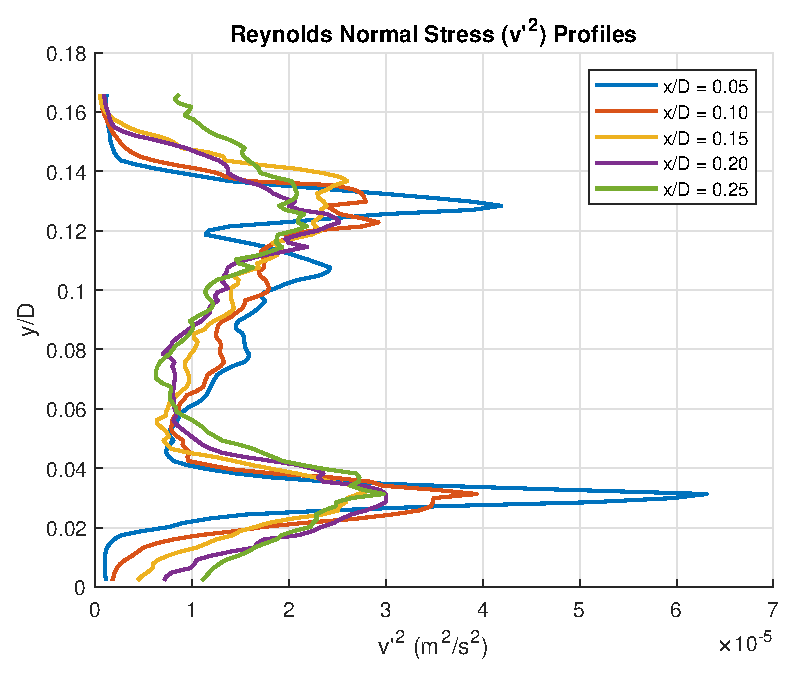
\includegraphics[width=0.9\textwidth]{vv_profiles_vs_y.eps}
    \caption{Reynolds normal stress in the $y$ direction, $\overline{v'^2}$, across multiple $x/D$ locations.}
    \label{fig:vv_profiles}
\end{figure}

\begin{figure}[H]
    \centering
    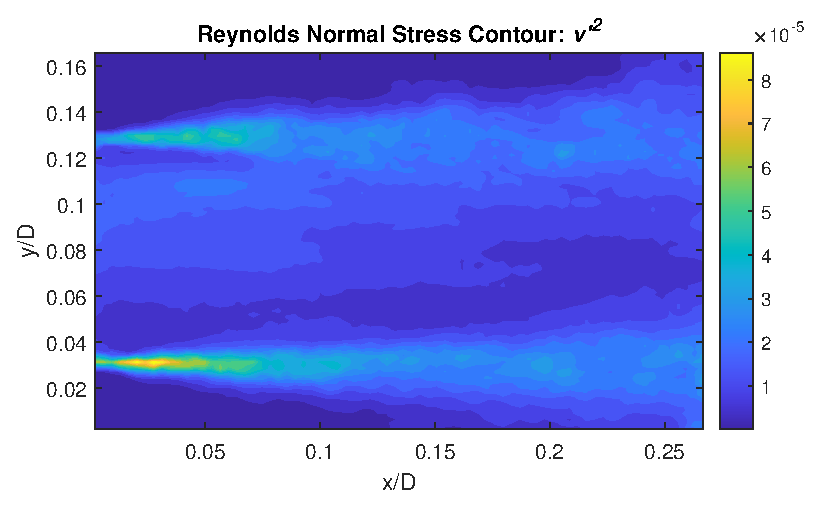
\includegraphics[width=0.95\textwidth]{vv_reynolds_normal_stress.eps}
    \caption{Contour of $\overline{v'^2}$, showing lateral turbulent intensity in the jet flow.}
    \label{fig:vv_contour}
\end{figure}

Each plot above is normalized spatially by nozzle diameter $D$. Reynolds stresses and vorticity were computed using time-resolved velocity fields as described in Section~\ref{sec:theory}.

\section{Discussion}

The contour plots and velocity profiles clearly illustrate the evolution of the round turbulent jet, including the presence of a potential core near the nozzle exit and shear layer development downstream. Reynolds normal and shear stress maps confirm that turbulence intensifies as the jet progresses, with peak values occurring around $x/D \approx 0.15{-}0.20$, consistent with literature predictions \cite{mattingly1962round, cooper2004round}.

One notable observation is the asymmetry in some of the Reynolds stress profiles, particularly in $u'v'$ and $v'^2$. This may be due to slight misalignments in the experimental setup or non-uniform lighting across the field. The vorticity magnitude plots also suggest the emergence of coherent vortical structures, highlighting the shear layer instabilities described in theoretical studies \cite{liu2025piv, zhao2010piv}.

\subsection*{Design Recommendations}

\begin{itemize}
    \item \textbf{Camera Mount Stability}: To reduce image jitter and improve vector quality, ensure the camera is mounted on a vibration-isolated platform. Any camera movement directly impacts vector consistency across time steps.
    
    \item \textbf{Seeding Uniformity}: While flow structures were visible, enhancing the uniformity of seeding particles—particularly near the nozzle—could improve correlation accuracy, especially for early jet development.
    
    \item \textbf{Illumination Balance}: Ensure the laser sheet maintains consistent intensity across the field. Areas closer to the fiber-optic source appeared slightly brighter, which could affect image pair matching.
    
    \item \textbf{Edge Padding in Data Processing}: To avoid artifacts introduced by missing data at the field edges, consider expanding the field of view or capturing higher-resolution vector grids for better post-processing interpolation.
\end{itemize}

Overall, the experiment effectively demonstrated key features of turbulent jet flow, and the proposed improvements would further enhance data quality and repeatability for future implementations.

\section{Conclusion}
This experiment successfully visualized and quantified the development of a turbulent round jet using Particle Image Velocimetry (PIV). Time-averaged velocity fields and Reynolds stress maps revealed a well-defined potential core and the growth of turbulence in the shear layer. Minor asymmetries in stress profiles and vorticity could be attributed to non-uniform seeding or illumination. These discrepancies highlighted the importance of setup precision and lighting uniformity in PIV-based measurements. Overall, the results validated key theoretical principles of jet flow and demonstrated a clear understanding of turbulence characteristics.

\section*{Acknowledgments}
The author would like to thank Dr. Xiaofeng Liu for his guidance and Teacher's Assistant Andrew Balolong for assistance during the experiment.

\bibliography{references}
\bibliographystyle{new-aiaa}

\section{Appendix}
\appendix

\section{Data Example}

Figure~\ref{fig:csv_sample} shows a screenshot of one of the 300 raw data files produced by the PIV system used in this experiment. Each file contains instantaneous velocity field data for a single image pair, with vector components recorded in both pixel units and meters per second. These files were processed using EduPIV and MATLAB to compute mean velocities, vorticity, and Reynolds stress components.

\begin{figure}[H]
    \centering
    \includegraphics[width=\textwidth]{EduPIV_lab.62tbxosb.000000.jpg}
    \caption{Sample raw data file from EduPIV output: \texttt{EduPIV\_lab.62tbxosb.000000.csv}}
    \label{fig:csv_sample}
\end{figure}

\section{Sample Calculation}
\label{app:samplecalc}

To demonstrate how time-averaged velocity components are calculated, consider the following single data point from \texttt{EduPIV\_lab.62tbxosb.000000.csv} (Figure~\ref{fig:csv_sample}):

\begin{table}[h!]
\centering
\begin{tabular}{cccc}
\toprule
x [mm] & y [mm] & $U$ [m/s] & $V$ [m/s] \\
\midrule
0.1086 & 0.1086 & 0.0007737 & 0.0031071 \\
\bottomrule
\end{tabular}
\caption{Sample Data Point at Grid Location from CSV file}
\end{table}

Assume the same data point is repeated for all 300 time steps (for illustration). Then, the time-averaged horizontal velocity at that location is:

\begin{align*}
\bar{u}(x_i, y_j) &= \frac{1}{N} \sum_{t=1}^{N} u(x_i, y_j, t) = \frac{1}{300} \cdot \sum_{t=1}^{300} 0.0007737 \\
&= 0.0007737 \text{ m/s}
\end{align*}

In practice, the MATLAB script \texttt{ImportData\_EduPIV.m} reads each CSV file and stores the $u$ and $v$ data in a 3D matrix. The time-averaged fields are computed using:

\begin{verbatim}
u_mean = mean(u_raw, 3, 'omitnan');
v_mean = mean(v_raw, 3, 'omitnan');
\end{verbatim}

This yields $\bar{u}(x_i, y_j)$ and $\bar{v}(x_i, y_j)$ across the entire field. These fields are then interpolated and plotted to visualize flow structures.


\section{MATLAB: Instructor Provided Code}
The following MATLAB script \cite{matlab} was provided by the instructor to analyze the raw lab data like the ones shown in Figure~\ref{fig:csv_sample}:
\lstinputlisting[language=Matlab, caption={Instructor provided MATLAB Code}]{ImportData_EduPIV.m}

\section{MATLAB: My Code}
The following MATLAB script \cite{matlab} was used for all Data Reduction and Graph Plotting:
\lstinputlisting[language=Matlab, caption={My MATLAB Code for Data Analysis}]{AE303_Lab6.m}

\end{document}